% !TEX TS-program = pdflatexmk

\documentclass{beamer}
\usepackage{times}
\usepackage{hyperref}
\usepackage{enumitem}

\mode<presentation>
{
  \usetheme{UAB}
  \setbeamercovered{transparent}
  \setbeamertemplate{headline}{}
  \setbeamertemplate{blocks}[rounded]
  \setbeamertemplate{navigation symbols}{}
}

\DeclareMathOperator*{\argmin}{argmin}
\DeclareMathOperator*{\argmax}{argmax}

\author{Steven Bethard}
\subject{CS 499: Senior Capstone}


\title{Social Inequality}
\date{}

\begin{document}

\begin{frame}
\titlepage
\end{frame}

\begin{frame}{Quiz}
The 2003 article by Jessica Brown reported that:
\begin{enumerate}[(A)]
\item<1> Of households making $<$\$15K, less than 5\% had internet access % No: 10%
\item<1> A low income white child was 2 times more likely to have internet access at home than a low income black child % No: 3 times
\item<1-2> Schools with 90\% minority children had 70\% higher student-to-computer ratios than average % 17-1 vs. 10-1
\item<1> Schools in high-income areas were twice as likely to have internet access as schools in low income areas % No: 75% vs. 55%
\end{enumerate}
\bigskip
The 2013 article by Jessica Goodman reported that:
\begin{enumerate}[(A)]
\item<1> 91\% of Americans have broadband at home % 71\%
\item<1> 66\% of 18-29 year-olds have a laptop; 57\% have a smartphone % reversed: 57% and 66%
\item<1-2> 98\% of the U.S. population has access to 3 Mbps downstream
%100 million people in the U.S. lived in areas where they had access to broadband, but did not subscribe
\item<1> $>$95\% of Fortune 500 companies require online job applications % 80%
\end{enumerate}
\end{frame}

\begin{frame}{Discussion}
\begin{itemize}
\item Who have you met that doesn't have internet access?
\bigskip
\item \href{http://www.openwifispots.com/FinderDirectoryCity.aspx?City=Birmingham&State=AL}{Where can you go for free internet access?}
\end{itemize}
\end{frame}

\begin{frame}{Decline of Print Media}
% http://www.theguardian.com/media-network/media-network-blog/2013/jan/02/end-newsweek-digital-evolution-rosenblum
\begin{columns}
\begin{column}{0.5\textwidth}
History:
\begin{itemize}
\item 1933 - Launched by former editor of Time
\item 1961 - Bought by Washington Post Company
\item 2009 - Refocused on opinion/commentary; 50\% decline in subscriptions
\item 2010 - Merged with online publication The Daily Beast
\item 2013 - End of US print versions
\end{itemize}
\bigskip
\uncover<2->{Does this affect the Digital Divide?}
\end{column}
\begin{column}{0.45\textwidth}
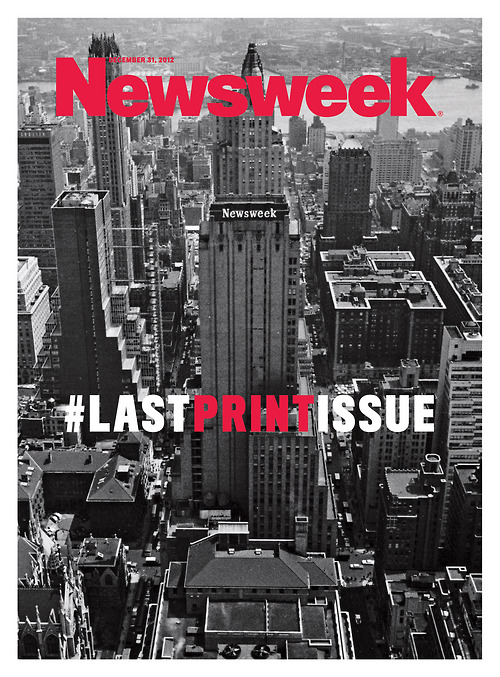
\includegraphics[width=\textwidth]{Newsweek_final_issue.jpg}
\end{column}
\end{columns}
\end{frame}

\begin{frame}{Digital Textbooks}
\href{http://www.youtube.com/watch?v=UB2RXPqFgdI}{A High School Without Textbooks}\\
\bigskip
How would the different factors interact with the Digital Divide?
\begin{itemize}
\item Cost to schools?
\item Cost to students?
\item Alternate learning strategies?
\item One-on-one interactions?
\item Weight of backpacks?
\item Social media distractions?
\end{itemize}
\end{frame}
\end{document}
